\documentclass[conference]{IEEEtran}
\IEEEoverridecommandlockouts
% The preceding line is only needed to identify funding in the first footnote. If that is unneeded, please comment it out.
\usepackage{cite}
\usepackage{amsmath,amssymb,amsfonts}
\usepackage{graphicx}
\usepackage{textcomp}
\usepackage{xcolor}
\def\BibTeX{{\rm B\kern-.05em{\sc i\kern-.025em b}\kern-.08em
    T\kern-.1667em\lower.7ex\hbox{E}\kern-.125emX}}

%%%%%%%%%%%%%%%%%%%%%%%%%%%%%%%%%%%%%%%%%%%%%%%%%%%
\usepackage[pdftex]{hyperref}


\usepackage{subcaption}
\usepackage{pdflscape}
\usepackage{pdfpages}
\usepackage{float}
\usepackage{multirow}
\usepackage[nottoc]{tocbibind}
\usepackage{afterpage}
\usepackage{tikz, lipsum,lmodern}
\usepackage{calligra,frcursive,xcolor}
\usepackage{pifont}
\usepackage[most]{tcolorbox}
\usepackage{fancyvrb}
\usepackage{array}
\usepackage{tabularx}
\usepackage{multirow}
\usepackage{pgfplots}
\usepackage{algpseudocode}
\usepackage{algorithm}
\usepackage{algorithmicx}

%%%%%%%%%%%%%%%%%%%%%%%%%%%%%%%%%%%%%%%%%%%%%%%%%%%
\usepackage{todonotes}
\newcommand{\revL}[1]{\textcolor{blue}{#1}}
\newcommand{\revR}[1]{\textcolor{purple}{#1}}
\newcommand{\revJ}[1]{\textcolor{red}{#1}}
\newcommand{\todoL}[1]{\todo[inline,color=blue]{LEO: #1}}
\newcommand{\todoR}[1]{\todo[inline,color=red]{RICARDO: #1}}
\newcommand{\todoJ}[1]{\todo[inline,color=purple]{JAVI: #1}}
%%%%%%%%%%%%%%%%%%%%%%%%%%%%%%%%%%%%%%%%%%%%%%%%%%%%%%


\begin{document}

% \title{A hybrid path planning strategy for the guidance of differential drive robots using rapidly exploring random trees in informed harvesting tasks.\\
\title{Efficient Hybrid Path Planning for Agricultural Robot-Assisted Harvesting operations.\\
\thanks{Identify applicable funding agency here. If none, delete this.}
}

\author{\IEEEauthorblockN{1\textsuperscript{st} Ricardo Urvina Córdova}
\IEEEauthorblockA{\textit{Universidad Católica del Norte} \\
\textit{Antofagasta, Chile} \\
ricardo.urvina@alumnos.ucn.cl}
\and
\IEEEauthorblockN{2\textsuperscript{nd} Leonardo Guevara}
\IEEEauthorblockA{\textit{Lincoln Institute for Agri-Food Technology (LIAT)} \\
\textit{Lincoln Centre for Autonomous Systems (L-CAS)} \\
\textit{University of Lincoln, UK} \\
lguevara@lincoln.ac.uk}
\and
\IEEEauthorblockN{3\textsuperscript{rd} Alvaro Prado}
\IEEEauthorblockA{\textit{Universidad Católica del Norte} \\
\textit{Antofagasta, Chile} \\
alvaro.prado@ucn.cl}
}

\maketitle
%%%%%%%%%%%%%%%%%%%%%%%%%%%%%%%%%%%%%%%%%%%%%%%%%%%%%%

\begin{abstract}
\textcolor{blue}{This article presents a path-planning strategy for autonomous mobile robots to guide scheduled harvesting tasks within expansive crop row fields of agricultural environments subject to terra-mechanical constraints. The proposed planner uses a two-stage approach, integrating a global planning strategy based on the Traveling Salesman Problem under the Capacitated Vehicle Routing approach, while a local planning methodology based on the Informed Rapidly-exploring Random Trees (RRT$^*$) subject to terrain constraints is devoted to connecting the previously scheduled harvesting points. The first approach is aimed at obtaining a queue waypoint list of harvesting locations, maximizing the amount of harvested product. In the second stage, the informed RRT$^*$ planner avoids environment obstacles in the robot configuration space and incorporates a kinematic model of a differential drive robot to meet kinematic constraints compatible with those of the designed path. Experimental results demonstrate the effectiveness of the proposed RRT$^*$ planner, achieving smooth and collision-free trajectories, making it suitable for practical applications in precision agriculture}.  
\end{abstract}

\begin{IEEEkeywords}
Path planning, Travel Salesmam Problem, Rapidly Random Exploring Tree, \revL{Agricultural robots}.
\end{IEEEkeywords}
%%%%%%%%%%%%%%%%%%%%%%%%%%%%%%%%%%%%%%%%%%%%%%%%%%%%%%

\section{Introduction}
\revR{Sugiero reducir el texto en el titulo, algo como Hybrid path planning for robot-assisted harvesting operations}
Path planning for \revL{autonomous} mobile robots in complex and constrained agricultural terrains is a critical and emerging area of research in robotics and automation, particularly in the context of Precision Agriculture (PA). 
%The increasing use of autonomous robotic systems in agriculture has created a growing demand for efficient and robust path-planning techniques \cite{Planas}. This need becomes especially \todoJ{pronounced} when considering the intricacies of PA, where fields are often organized into multiple rows. 
For differential drive robots (DDR) \revR{Sugiero reemplazar el termino "differential drive" por "differential drive"}, path planning introduces distinctive challenges due to their limited mobility and potential instability on uneven terrain \cite{Auat2017}. Developing a path planner that caters to the nuances of multi-row crop fields, while considering terrain constraints, dynamic obstacles, and optimizing paths for DDR, is essential for realizing their full potential in real-world agricultural scenarios \cite{FAO2050}.

Existing path planning approaches vary in their ability to account for the robot's kinematics and the terrain's traversability. Traditional methods, such as Dijkstra's algorithm and A* search, focus on finding the shortest path in terms of distance, often neglecting the robot's dynamic constraints \cite{Pak2022}. While these methods perform well in certain scenarios, they may lead to infeasible paths for DDR, hampering their navigation and efficiency.

Recent advancements in path planning introduce techniques that incorporate the robot's kinematic model and consider terrain traversability to generate more feasible and optimized paths \cite{Xie2020}. Some planners \cite{Mashayekhi2020, Kontoudis2019,Zhang2019,Denggui } employ Rapidly-exploring Random Trees (RRT) or RRT variants, which efficiently explore the configuration space while taking dynamic constraints into account. Nevertheless, these methods may lack the capability to ensure kinematic feasibility, potentially resulting in paths that exceed the robot's physical limitations.

Another aspect to consider in path planning is the optimization of paths for multiple objectives, such as minimizing energy consumption or maximizing mission success rates \cite{Janos2021}. The Traveling Salesman Problem with Capacitated Vehicle Routing (TSP-CVRP) is a widely adopted approach to optimize paths for multiple vehicles, ensuring efficient load distribution and reducing overall travel distance \cite{Milos2022},\cite{Dereci2022}. Integrating TSP-CVRP with local exploration techniques can offer a comprehensive \todoL{No creo que "compehensive" sea un termino adecuado para describir tu solucion, esto lo repites un poco mas abajo} solution that combines global optimality with local adaptability for path planning.

Motivated by the unique challenges posed by DDR, \todoL{No entiendo esta parte, cual fue tu motivacion para trabajar con vehiculos uniciclo? para mi la razon principal es que esta clase de configuracion es la mas tipica en robots de tamano mediano ya que su control es sencillo, y los costos de manofactura son minimos comparados a car-like o 4WS.} this research aims to propose a comprehensive path planning algorithm that takes into account the robot's kinematics and terrain traversability. \todoL{Todo el parrafo que sigue debe ser reescrito (bastantes errores gramaticales). Como parece que esto es una etapa importante de tu metodologia, deberias incluir algunas referencias de trabajos relacionados a generacion de mapas aereos para generacion de rutas. En tu caso, deberias dejar claro que la generacion de mapa (que incluye la extraccion de costmap, collection points, y traversability map) forma parte de la etapa inicial de tu proceso de generacion de rutas.} In addition to these considerations, this study also involves the processing of a field map. A map of the simulation was constructed in Coppelia V-REP, simulating a multi-row crop field. The field was processed using a vision sensor, and the obtained data were analyzed to process the image. The data set thus obtained was used to identify harvest points, obstacles within the map, and possible slip.

By incorporating the TSP-CVRP approach for global planning and informed RRT for local exploration, the proposed method seeks to strike a balance between path quality and computational efficiency. Furthermore, the integration of the DDR kinematic model ensures that the generated paths are both feasible and dynamic compatible with the robot's limitations.

The primary objective of this study is to develop a path planner that can efficiently generate optimized paths for DDR in complex environments. The planner will take into consideration dynamic \todoL{Si solo estas ocupando el modelo cinematico, trata de evitar usar el termino "dynamic".} robot constraints, terrain traversability, and multiple objectives, aiming to enhance the overall performance and reliability of DDR in various applications. Through simulation studies and performance evaluations, this research will demonstrate the effectiveness and advantages of the proposed path planner compared to existing state of the art methods.

In the subsequent sections, the paper delves into the foundation and context of the research in the Section \ref{Sec::state_art} The Section \ref{Sec::materials} presents the tools, data, and experimental setup that underpin the investigation. Followed by Section \ref{Sec::methdology} details the step-by-step approach employed to address the research work. In Section \ref{Sec::results} presents the outcomes, and finally, in Section \ref{Sec::conclusions} the discussion revolves around the implications and significance of the findings.

%%%%%%%%%%%%%%%%%%%%%%%%%%%%%%%%%%%%%%%%%%%%%%%%%%%%%%
\section{State of the art}
\label{Sec::state_art}
Path planning algorithms provide solutions aimed at optimality for problems in various domains. These algorithms can be implemented for aerial, maritime, and terrestrial vehicles \cite{Yu2021,Xie2020}. There are several elements within navigation systems that directly influence the route planning system. The key considerations for developing a route planner are: I) the navigation environment, II) the robot's kinematics, and III) the general problem to be solved. It is important to note that different planning algorithms are adaptable and can be combined with other non-planning algorithms. Furthermore, certain algorithms, such as RRT, allow for the integration of external models that, in conjunction, yield a smoother route \cite{Chen2020}. A smooth route is one in which a robot, when provided with a path, can complete the trajectory while considering its kinematic conditions.

Robots have become increasingly common in PA. Despite significant research progress in the field of path planning in recent years, there are still outstanding challenges to address. For instance, many path planners primarily focus on minimizing route length, often overlooking the maximization of other objectives that could be integrated into the path planning process \cite{Dereci2022}. In the work by Auat et al. \cite{Auat2017}, path planning strategy takes into account the robot's kinematic constraints while considering terramechanical limitations. This contribution presents an integrated strategy for harvest and motion planning, utilizing crop yield information. Harvesting locations are formulated as a Traveling Salesman Problem (TSP), while motion planning is addressed using the RRT* algorithm, which incorporates terrain traversability. However, this work raises several concerns:

\begin{enumerate}
  \item Only 5\% effort savings were achieved when using RRT* with terrain constraints compared to using RRT* without terrain restrictions.
  \item Cumulative path tracking error showed no substantial difference between RRT* with and without terrain constraints.
\end{enumerate}

Given the aforementioned challenges, there is a need to develop a path planner that can enhance the results obtained by \cite{Auat2017}. This research aims to demonstrate that path planning can be achieved in fewer iterations and less time while maintaining the same conditions. This improvement should reduce cumulative errors, accounting for terrain constraints and robot skidding.

According to Xu et al. in \cite{Xu2020}, the planning speed of the RRT algorithm is slow, and the path planning failure rate using the PRM algorithm is high in complex scenarios. The authors propose the fusion of PRM and bidirectional RRT based on probability (P-Bi-RRT), which divides the planning area into two equally sized regions on average. The PRM algorithm with faster planning speed is used to prepare the route in each area, followed by selecting one node from each region to form an optimal pair of matching points. These points are then used to connect the two regional routes. The authors demonstrated that path planning time was reduced by 71\% to 80\%, the number of nodes was reduced by 70\% to 80\%, and path length was shortened by 20\% to 30\% compared to the RRT algorithm.

Efficient exploration of the environment using random points during the RRT algorithm is a frequent problem in path construction. Therefore, Chen et al. in \cite{Chen2020} propose a hybrid RRT method incorporating machine learning techniques. This method simultaneously generates a global tree and a local tree to explore boundary points. Detected boundary points are filtered using the DBSCAN clustering method, resulting in a set of target points used as the current target point for robot movement. The algorithm comprises five components: i) boundary point exploration based on RRT, ii) boundary point filtering with DBSCAN, iii) target distribution, iv) planning, and v) route construction. It is recommended to employ a hybrid RRT* method with unsupervised machine learning techniques.

It is noteworthy that many path planners in agriculture do not adequately consider the robot's kinematic and dynamic constraints, often leading to paths that the robot cannot traverse. However, this issue was addressed in the late 1990s \cite{Auat2017}. Another aspect frequently overlooked by path planners is terrain traversability, given that wheel-terrain interaction plays a fundamental role in robot mobility over uneven terrains. Considering terramechanical terrain features allows robots to adapt their control and planning strategy to minimize energy consumption \cite{Ding}. Wheel slippage is a common problem in rough terrains and is related to soil terramechanical properties. Various empirical methods have been used to determine soil resistance, such as the cone index and maximum mean pressure \cite{ALMILLI2010151}. These methods offer a straightforward means of evaluating mobility based on a "pass/fail" criterion.

Based on Papadakis \cite{Papadakis2013}, most empirical models were developed to assess soil penetration resistance. Papadakis points out two ways to estimate terrain traversability without physical interaction with the terrain:

\begin{enumerate}
  \item Geometry-based (point clouds with LiDAR, elevation maps).
  \item Appearance-based (RGB images, multispectral images).
\end{enumerate}

Various mathematical models are available to predict wheel-terrain interaction based on terrain properties and wheel characteristics. Some of the most common models are:

\begin{itemize}
  \item Coulomb Model \cite{Ding}: Based on Coulomb's law to calculate the wheel-terrain friction force.
  \item Spencer Model: Based on Mohr-Coulomb theory \cite{Massoudi} to calculate friction force based on soil tension.
\end{itemize}

Each of these models has its own advantages and disadvantages in terms of precision and complexity. Most works studying soil properties rely on a set of tests proposed by Bekker \cite{bekker1956theory}, known as the Bevameter Technique, which led to the development of pressure-sinkage and traction-slippage relationship models. Wong further expanded these models to allow the prediction of track resistance, traction effort, and slip for a track based on soil properties \cite{Wong}.

% as shown in Equations 1 and 2 by \cite{ALMILLI2010151}

% \begin{equation}
% R_{c}=\dfrac{bl}{(n+1)(\dfrac{k_{c}}{b+k_{\phi}})} * (\dfrac{W}{bl})^{(\dfrac{n+1}{n})}
% \end{equation}

% \begin{equation}
% F=(A_{c}+W\tan(\phi))[1+\dfrac{k}{il}(1-e^{-(\dfrac{il}{K})})]
% \end{equation}

% where \(R_{c}\) represents road motion resistance due to soil compaction, and \(k_{c}\), \(k_{\phi}\), and \(n\) are the pressure sinkage parameters. \(W\) stands for vehicle weight, \(l\) and \(b\) denote the length and width of contact of the track, respectively. \(F\) represents total traction, \(A\) is the track contact area (\(A = b \cdot l\)), \(c\) is cohesion, \(\phi\) represents the friction angle, \(K\) is the shear modulus, and \(i\) is the longitudinal slip of the track. These models have been applied in various works, such as terrain traversability modeling through reinforcement learning incorporating exteroceptive and proprioceptive sensor data \cite{GanLu}, and terrain traversability analysis for unmanned ground vehicles \cite{Papadakis2013}. These works identify that the core of all these methodologies uses 3D terrain information acquired through light sensors, stereo range data, color images, or other sensor data, occasionally combined with static or dynamic modeling of vehicle-terrain interaction.

In \cite{Milos2022}, a generalized exploration of unknown environments by autonomous mobile robots is conducted, where a robotic agent learns terrain traversability and constructs a spatial model of the environment. After reviewing the literature, it is found that few works conduct path planning considering both the robot's dynamic constraints and the terrain constraints encountered in agriculture.

There are various kinematic and dynamic models developed for off-road vehicles. However, these models have been simplified into empirical formulas, rendering them useless for online predictions \cite{ALMILLI2010151}. 
% This work adopts the dynamics and kinematics models by Bekker and Wong \cite{bekker1956theory}, \cite{Wong} for predicting the traversability and maneuverability performance of Skid-Steer differential drive-type vehicles.

%%%%%%%%%%%%%%%%%%%%%%%%%%%%%%%%%%%%%%%%%%%%%%%%%%%%%%

\section{Materials and Methods}
\label{Sec::materials}

This section outlines the components of the research methodology, encompassing the simulation environment, the construction of a 3D map within Coppelia V-REP simulating multi-row crop fields, the image processing employed, and the results achieved through this processing. These elements collectively form the foundation for our comprehensive path planning algorithm designed to address the complexities of PA in multi-row crop fields, with a focus on DDR. \todoL{Aqui creo que seria bueno incluir una grafica general de bloques con todos los componentes de tu propuesta de generacion de caminos, cada bloque debe coincidir con los nombres de las subsecciones.}

\subsection{Robotics Simulation Platform}
The use of different simulators and virtual environments for testing robotic designs is a topic of interest. In \cite{Ramin2018} is presented a comparative study that evaluates the performance of VREP, Gazebo, and ARGoS simulators across various scenarios, from small to large scenes with changing robot numbers.

Results indicate that VREP has slower simulation speeds and higher memory usage compared to the other two simulators. In contrast, ARGoS exhibits faster simulation in small scenes, while Gazebo becomes more efficient as scene complexity increases. Notably, V-REP's performance can be significantly improved through careful parameter configuration and model optimization, as observed in reference [18].

V-REP offers an extensive feature set, including a scene editor, 3D model import capabilities, and mesh manipulation. However, it has a limitation in defining scenes using XML files.

\begin{figure}[t!]
	\centering
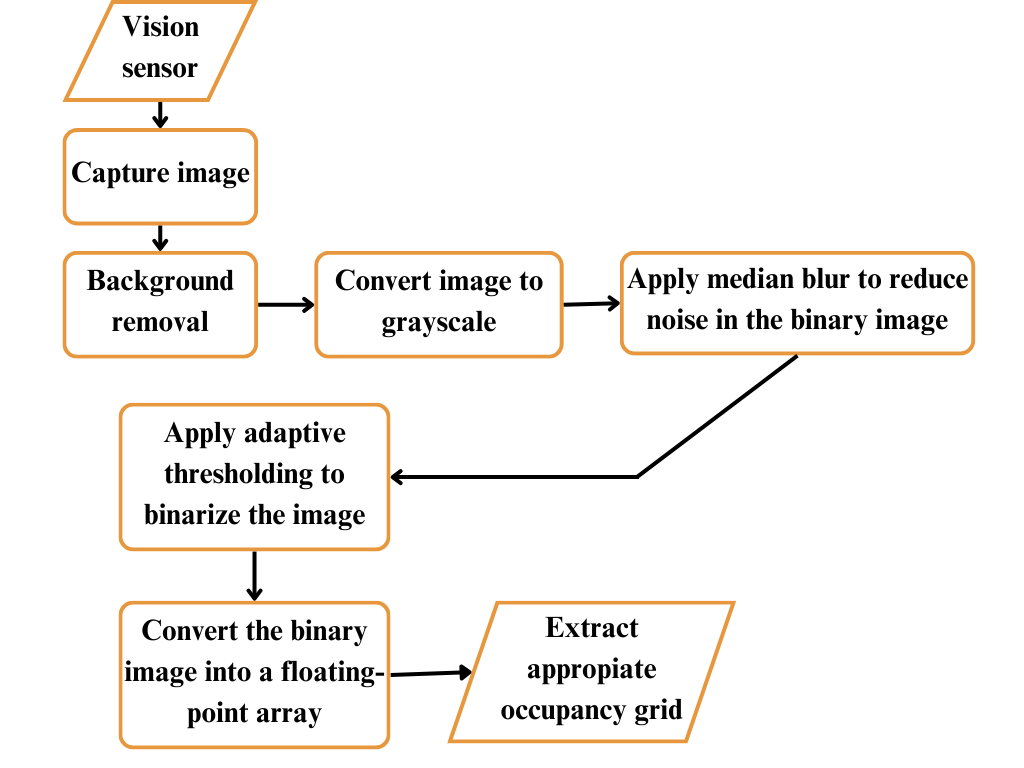
\includegraphics[width=100mm]{Images/EnvironmentDevelopmentPipeline.png}
\caption{Environment development pipeline}
\label{Fig::EnvironmentDevelopmentPipeline}
\end{figure}

\subsection{Rendeing of the navigability map}
The image processing algorithm for crop detection involves six steps. Figure \ref{Fig::EnvironmentDevelopmentPipeline} provides a bried overview of the methdology applied to process the image. Initially, a vision sensor captures an image, which is then subjected to background removal to isolate relevant features. The image is subsequently converted to grayscale ($I_{gray}$). To minimize noise within the binary image, a median blur operation is applied, which can be expressed as:


\begin{equation}
I_{blurred} = \text{MedianBlur}(I_{gray}, k)
\end{equation}

where $k$ represents the kernel size for the median blur filter. Following this, adaptive thresholding is employed to binarize the blurred image. This operation can be described as:

\begin{equation}
I_{b} = \text{AdaptiveThreshold}(I_{blurred}, \text{blockSize}, \text{C})
\end{equation}

where $I_{b}$ represents the binary image, \textit{blockSize} is the size of the local neighborhood, and \textit{C} is a constant subtracted from the mean. The binary image is subsequently converted into a floating-point array, yielding a matrix $M_{float}$. Finally, from this matrix, an appropriate occupancy grid is extracted.

The mapping enables a precise assessment of crop distribution, which plays a pivotal role in optimizing harvest operations. In Figure \ref{fig:rgb1}, the simulated map is presented, and in Figure \ref{fig:occupancy_grid1}, the map after the performed processing is shown.

\begin{figure*}[t!]
    \begin{minipage}{0.5\textwidth}
        \centering
        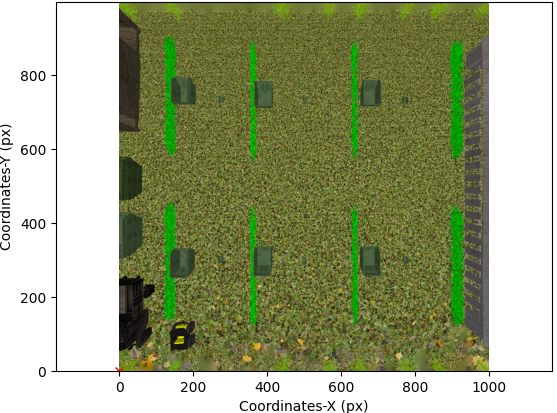
\includegraphics[width=\linewidth]{Images/rgb1.png}
        \caption{Simulation of an agricultural environment with 8 rows and 8 harvest points}
        \label{fig:rgb1}
    \end{minipage}\hfill
    \begin{minipage}{0.5\textwidth}
        \centering
        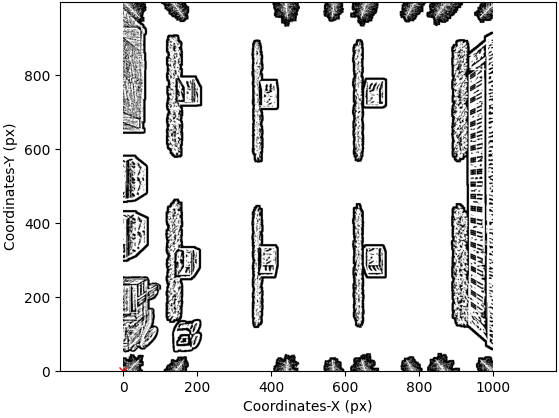
\includegraphics[width=\linewidth]{Images/occupancy_grid1.png}
        \caption{Processed image converted to occupancy grid forma}
        \label{fig:occupancy_grid1}
    \end{minipage}
\end{figure*}

\subsection{Model of the differential drive robot}
\subsection{Model of the terrain traversability}
%%%%%%%%%%%%%%%%%%%%%%%%%%%%%%%%%%%%%%%%%%%%%%%%%%%%%%
\section{Methodology}
\label{Sec::methdology}

The proposed work will be developed through an experimental methodology to fulfill the specific objectives. Next, the proposed methodology follows 5 stages as shown in Fig. \ref{Fig::esquema_basico_planificacion}

\begin{figure*}[t!]
	\centering
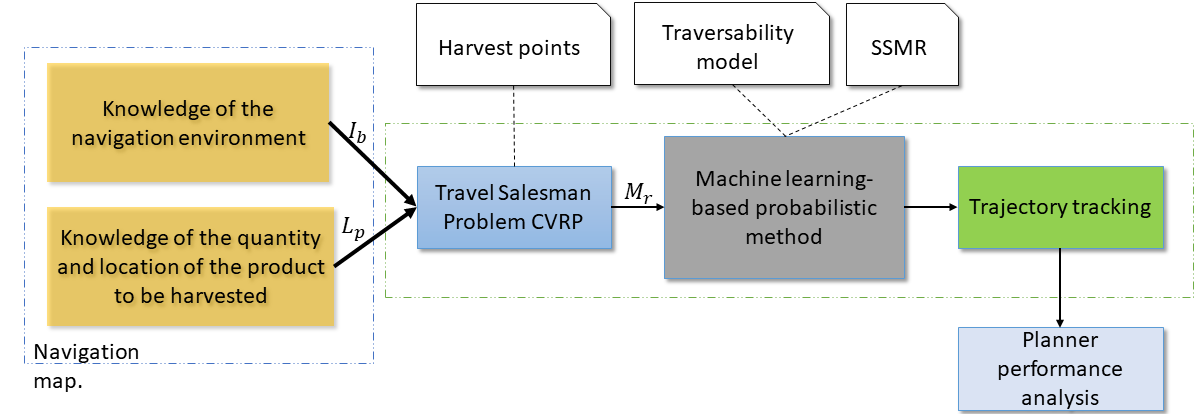
\includegraphics[width=165mm]{Images/esquema_basico_planificacion.png}
	\caption{General scheme of the integrated global and local planning Skid-Steer Mobile Robots (SSMR) under tearrain constraints.}
	\label{Fig::esquema_basico_planificacion}
\end{figure*}

A navigation map is a graphical representation of an environment used to plan and guide an agent's movement within that environment. These maps typically include information about the space's geometry, the presence of obstacles and other elements that can affect navigation, as well as points of interest and preferred routes. The generation of a navigability map simulating a crop field is considered, where objects, collection points, and terrain traversability are presented. A navigability map \(M\) was defined as a tuple \((G, O, C)\), where:
\begin{itemize}
\item \(G = (V, E)\) is an undirected graph representing the search space; \(V\) is the set of nodes corresponding to discretized points in space, and \(E\) is the set of edges representing connections between nodes and possible paths between them.
\item \(O \subseteq V\) is the set of nodes corresponding to obstacles in space.
\item \(C: V \times V \to \mathbb{R}\) is a cost function assigning a value to each pair of nodes \((u, v) \in V \times V\), representing the cost or difficulty of following a path from node \(u\) to node \(v\).
\end{itemize}

In the conducted experiments, a 15 x 15-meter map was employed, comprising 6 collection rows. Each row has a width of 4 meters and a length of 3 meters and Each collection row features a designated waypoint to which the robot is tasked to navigate for crop harvesting. The presence of obstacles within the map and areas susceptible to slippage is considered.


\subsection{Travel Salesman strategy with Capacitated Vehicle Routing Problem}
The Capacitated Vehicle Routing Problem (CVRP), can be defined as a graph $G = (N, E)$, where $N$ is the set of ordered harvest points $\{0, 1, . . . , n\}$. Node $0$ represents the depot, and nodes $\{1, . . . , n\}$ represent the harvest points (HP). Each edge $\{i, j\} \in E$ is associated with a non-negative cost $c_{ij}$. Every HP $i \in V' = V \setminus \{0\}$ has a specific demand $q_i$, where $i = 1, 2, . . . , n$. A single depot, denoted as $0$, dispatches one vehicle $K$, it has a capacity limit of $Q$. This vehicle departs from the depot to serve each HP and then return. It's essential to note that the loading of each vehicle should not surpass the specified capacity limit $Q$. The main objective is to determine the optimal routes to fulfill all customer demands while minimizing the total routing cost. The CVRP can be mathematically formulated as follows:

\begin{align*}
\text{Minimize:} & \ \\
& \sum_{i=1}^{n}\sum_{j=1}^{n} d_{ij} x_{ij} \ \\
\text{Subject to:} & \ \\
& \sum_{j=1}^{n} x_{ij} = 1 \quad \forall i = 1, 2, ..., n \ \\
& \sum_{i=1}^{n} x_{ij} = 1 \quad \forall j = 1, 2, ..., n \ \\
& \sum_{j=1}^{n} w_j x_{ij} \leq Q \quad \forall i = 1, 2, ..., n \ \\
& x_{ij} \in {0, 1} \quad \forall i, j = 0, 1, 2, ..., n \ \\
& x_{ij} = 0 \quad \forall (i,j) \notin C \
\end{align*}


\noindent where $d_{ij}$ represents the distance between point i and point j.
$x_{ij}$ is a binary variable indicating whether there is travel from point i to point j.
$w_j$ is the weight associated with point j.
$K$ is the number of available vehicles.
$Q$ is the maximum capacity of each vehicle.
$C$ is the set of connections between specific points that must be adhered to.
\subsubsection{Solution representation. No necesitas esta subsección}
The TSP CVRP operates on various input parameters, including an occupancy grid ($O_{g}$), matrices of visiting points ($M_{pos}$) and weights ($M_{w}$), the maximum vehicle capacity ($Q$), and a dictionary of sections and objects ($Rows$). The algorithm initializes and retrieves essential data, including the environment data, distance matrix ($D_{m}$), and forbidden connections matrix ($F_{c}$). It also maintains variables like the collection sum ($S_{w}$).

The algorithm \ref{Alg::TSP} starts at the depot ($M_{pos}[0]$) and explores unvisited points to create a solution. It uses the PATH CHEAPEST ARC strategy to find the nearest unvisited point ($M_{pos}[i+1]$) from the current point ($M_{pos}[i]$). It checks if there are any forbidden connections ($F_{c}$) between points and ensures that the weight of the collection ($S_{w}$) does not exceed the vehicle's capacity ($Q$). If these conditions are met, the algorithm proceeds to create a solution ($S$). The process continues until all points are visited.

Finally, the algorithm applies a tabu search algorithm to obtain an ordered matrix of point positions ($M_{ord}$) for efficient routing.

\begin{algorithm}[t!]
\caption{TSP CVRP}
\label{Alg::TSP}
\begin{algorithmic}[1]
\Require
\State $O_{g} \gets$ Occupancy Grid
\State $M_{pos} \gets$ Visiting Points Matrix
\State $M_{w} \gets$ Matrix of weights
\State $Q \gets$ Maximum vehicle capacity
\State $Rows \gets$ Dictionary of sections and objects
\Ensure
\State Ordered matrix of visiting point positions
\State \textbf{Initialize} $Data $ = getDataEnvironment() \Comment{Retrieve positions, weights, and rows of the objects}
\State \textbf{Initialize} $D_{m} $ = getDistances($Data$) \Comment{Obtain distance matrix}
\State \textbf{Initialize} $F_{c} $ = getForbiddenConnections($Rows$) \Comment{Obtain restrictions matrix}
\State \textbf{Initialize} $S_{w} \gets$ 0 \Comment{Collection sum}
\State Start at $M_{pos}[0]$ and mark all $M_{pos}[i]$ as unvisited
\While{there are to visit}
\State \textbf{Apply} PATH CHEAPEST ARC
\State Find the nearest $M_{pos}[i+1]$ to the current $M_{pos}[i]$ that has not been visited yet.
\If{$M_{pos}[i+1]$ and $M_{pos}[i]$ are not in $F_{c}$}
\If{$S_{w} \leq Q$}
\State Go to the nearest $M_{pos}[i]$ and mark the current $M_{pos}[i]$ as visited.
\State $S_{w} \gets$ sum of $M_{w}[i]$
\State $S \gets$ \textbf{PATHCHEAPESTARC} \Comment{Obtain the first solution}
\EndIf
\EndIf
\EndWhile
\State $M_{ord} \gets$  \textbf{TABUSEARCH(S)} \Comment{Ordered matrix of harvest points}
\end{algorithmic}
\end{algorithm}

\subsection{Learning based rapidly-exploring random tree}
The RRT-Informed* with DDR Model Integration algorithm, as presented in Algorithm \ref{Alg::rrt-unycle}, is designed to find a feasible path for a DDR from a given start state to a goal state. It operates in an environment represented by an occupancy grid, which models obstacles and free spaces. This algorithm combines the principles of RRT* for efficient exploration and the integration of a DDR model to ensure that the generated paths are feasible for the robot.

\subsubsection{Integration of differential drive robot Model}
RRT* \cite{Qi2021} is an incremental, sampling-based planner with guaranteed asymptotic optimality, originally developed for holonomic systems. The algorithm \ref{Alg::rrt-unycle}, \ref{Alg::ChooseParent}, \ref{Alg::ReWire} is an extension of RRT* for DDR, using the steering and distance functions. It solves the optimal path planning problem by growing a tree $T = (V, E)$ with a vertex set $V$ of poses connected by edges $E$ of feasible path segments to find a path that connects exactly to the destination pose with minimum cost, using a set of basic procedures described below. $X$ is the configuration space of the vehicle, and $x: [0, 1] \to X$ is a path in the configuration space. The notations generally follow the RRT* algorithm presented in \cite{Qi2021}. Where is characterized by the following functions: i) The sampling process samples a pose $z_{\text{rand}} \in X_{\text{free}}$ from the obstacle-free region of the configuration space. The sampling is random with a goal bias, with which the destination pose is sampled to ensure that the path exactly connects to the destination pose. The distance function $\text{Dist}(z, z_0)$, as defined in eq. \ref{Eq::diste} , returns the non-holonomic directed distance from a pose $p = (x, y, \theta)^T$  to a target pose  $p_{0}$

\begin{equation}
\label{Eq::diste}
   \text{Dist}(p, p_0) = l(T_{p_0}((x, y, \theta)^T))
\end{equation}


\noindent iii) The cost function $c(z, z_0)$ measures the cost of the path from a pose $z$ to a pose $z_0$. In this paper, it is finded the minimum-distance path, so $c(z, z_0) = \text{Dist}(z, z_0)$. $Cost(v)$ returns the accumulated cost of a node $v \in V$ in the tree from the root. iv) The Nearest Neighbor give a pose $z \in X$ and the tree $T = (V, E)$, $v = \text{Nearest}(T, z)$ returns the node in the tree where the distance from the node to the pose $\text{Dist}(v, z)$ is minimum. v) The Nearby Nodes function give a pose $z$, tree $T = (V, E)$, and a number $n$, then:

\begin{equation}
\label{Eq::nearto}
    \text{NearTo}(T, z, n) \equiv \{v \in V \, | \, \text{Dist}(v, z) \leq L(n)\}
\end{equation}

\noindent where $L(n) = \gamma \left( \frac{\log(n)}{n} \right)^{1/d}$ with a constant $\gamma$ and the dimension of the space $d$ \cite{Fernandez2019}. This returns a set of nodes from which the distance to the pose $z$ is small.Similarly, 
\begin{equation}
\label{Eq::nearfrom}
   \text{NearFrom}(T, z, n) \equiv \{v \in V \,|\, \text{Dist}(z, v) \leq L(n)\} \quad
\end{equation}
returns the set of nodes that is near to the pose $z$. This distinction between \texttt{NearTo()} and \texttt{NearFrom()} is necessary due to the use of directed distance. vi) The Steering funcion is assumed that the vehicle follows the vector field, e.g., the feedback control on the heading $\delta^*$. Then $x = \text{Steer}(z, z_0)$ which generates a path segment $x$ that starts from $z$ and ends exactly at $z_0$, and $(z_{\text{new}}, x_{\text{new}}) = \text{Extend}(z, z_0, \varepsilon)$ starts from $z$ and extends the path toward $z_0$ until $z_0$ is reached or the distance covered is $\varepsilon$, and returns the new sample $z_{\text{new}}$ at the end of the extension. \text{Extend}() is a standard RRT procedure for exploration. These functions are described in Algorithms \ref{Alg::rrt-unycle}, \ref{Alg::ChooseParent}, \ref{Alg::ReWire}.


\begin{algorithm}
\caption{ $T =(V,E) \leftarrow$ Differential drive RRT* ($z_{init}$)}
\label{Alg::rrt-unycle}
\begin{algorithmic}[1]
\State $T  \leftarrow$ InitializeTree();
\State $T \leftarrow$ InsertNode$(\emptyset, z_{\text{init}}, T)$;
\For{$i = 1$ to $N$}
    \State $z_{\text{rand}} \leftarrow$ Sample$(i)$;
    \State $z_{\text{nearest}} \leftarrow$ Nearest$(T, z_{\text{rand}})$;
    \State $(z_{\text{new}}, x_{\text{new}}) \leftarrow$ Extend$(z_{\text{nearest}}, z_{\text{rand}}, \epsilon)$;
    \If{ObstacleFree$(x_{\text{new}})$}
        \State $Z_{\text{nearTo}} \leftarrow$ NearTo$(T, z_{\text{new}, |V|})$;
        \State $z_{\text{min}} \leftarrow$ ChooseParent$(Z_{\text{nearTo}}, z_{\text{nearest}}, z_{\text{new}})$;
        \State $T \leftarrow$ InsertNode$(z_{\text{min}}, z_{\text{new}}, T)$;
        \State $Z_{\text{nearFrom}} \leftarrow$ NearFrom$(T, z_{\text{new}, |V|})$;
        \State $T \leftarrow$ ReWire$(T, Z_{\text{nearFrom}}, z_{\text{min}}, z_{\text{new}})$;
    \EndIf
\EndFor
\State \textbf{return} $T$
\end{algorithmic}
\end{algorithm}

\begin{algorithm}
\caption{$z_{\text{min}} \leftarrow$ ChooseParent( $Z_{nearFrom}$,  $Z_{nearest}$,  $Z_{new}$)}
\label{Alg::ChooseParent}
\begin{algorithmic}[1]
\State $z_{\text{min}} \leftarrow z_{\text{nearest}};$
\State $c_{\text{min}} \leftarrow \text{Cost}(z_{\text{nearest}}) + c(z_{\text{nearest}}, z_{\text{new}});$
\For{$z_{\text{near}} \in Z_{\text{nearTo}}$}
    \State $x_0 \leftarrow \text{Steer}(z_{\text{near}}, z_{\text{new}});$
    \If{ObstacleFree($x_0$)}
        \State $c_0 \leftarrow \text{Cost}(z_{\text{near}}) + c(z_{\text{near}}, z_{\text{new}});$
        \If{$c_0 < \text{Cost}(z_{\text{new}})$ and $c_0 < c_{\text{min}}$}
            \State $z_{\text{min}} \leftarrow z_{\text{near}};$
            \State $c_{\text{min}} \leftarrow c_0;$
        \EndIf
    \EndIf
\EndFor
\State \textbf{return} $z_{\text{min}};$
\end{algorithmic}
\end{algorithm}

\begin{algorithm}
\caption{$T \leftarrow$ ReWire($T$, $Z_{nearFrom}$, $z_{min}$, $z_{new}$)}
\label{Alg::ReWire}
\begin{algorithmic}[1]
\For{$z_{\text{near}} \in Z_{\text{nearFrom}} \setminus \{z_{\text{min}}\}$}
    \State $x_0 \leftarrow \text{Steer}(z_{\text{new}}, z_{\text{near}});$
    \If{ObstacleFree($x_0$) and Cost($z_{\text{new}}$) + $c(z_{\text{new}}, z_{\text{near}}) < \text{Cost}(z_{\text{near}})$}
        \State $T \leftarrow \text{ReConnect}(z_{\text{new}}, z_{\text{near}}, T);$
    \EndIf
\EndFor
\State \textbf{return} $T;$
\end{algorithmic}
\end{algorithm}

% \begin{algorithm}
% \label{Alg::rrt}
% \caption{Loop RRT-Informed* for differential drive Robot}
% \begin{algorithmic}[1]
% \Require
% \State Start state $start = [x_{\text{start}}, y_{\text{start}}, \theta_{\text{start}}]$
% \State Goal state $goal = [x_{\text{goal}}, y_{\text{goal}}, \theta_{\text{goal}}]$
% \State Occupancy grid $occupancy\_grid$
% \State Random sampling area $rand\_area = [min\_value, max\_value]$
% \State Maximum iterations $max\_iter$
% \State Connection circle distance $connect\_circle\_dist$
% \State Robot radius $robot\_radius$
% \Ensure
% \Statex Flag $flag$ \Comment{Se posiciones, pesos y files de los objetos}
% \State Trajectory $x$, $y$, $yaw$ of the robot
% \State Speed $v$
% \State Time $t$
% \State Acceleration $a$
% \State Steering angle \(d\)

% \Function{RRT-Informed}{$start, goal, occupancy\_grid, rand\_area, max\_iter, connect\_circle\_dist, robot\_radius$}
%     \State Initialize planning parameters
%     \State Create an RRT* tree
%     \State Set target speed, yaw threshold, and tracking parameters
%     \State Initialize variables for the best feasible path
%     \State Perform RRT* planning with Reeds-Shepp paths
%     \State Generate a course based on the goal
%     \State Search for the best feasible path among the generated courses
%     \State Return the best feasible path
% \EndFunction

% \Function{GenerateFinalCourse}{$x$}
%  \State Generate a final path from the goal index
%     \State Return the path
% \EndFunction

% \Function{ExtendPath}{$cx$, $cy$, $cyaw$}
%     \State Extend the path to increase resolution
%     \State Return the extended path
% \EndFunction

% \Function{CheckCollision}{$node$}
%    \State Check if the path represented by the node is collision-free
%     \State Return true if collision-free, false otherwise
% \EndFunction

% \Function{Check}{$path$}
%  \State Prepare path points
%     \State Generate a speed profile
%       \State Perform closed-loop prediction using pure pursuit
%     \State Check if the goal can be reached
%     \State Check if the final angle is acceptable
%     \State Check if the path length is within limits
%     \State Check if the path is collision-free
%     \State Return whether the path is feasible
% \EndFunction

% \Function{CalcDistToGoal}{$x$, $y$}
%     \State Calculate the Euclidean distance to the goal
%     \State Return the distance
% \EndFunction


% \end{algorithmic}
% \end{algorithm}



\subsection{Trajectory Tracking}
\subsection{Planner performance analysis}
\section{Results}
\label{Sec::results}

\section{Conclusions}
\label{Sec::conclusions}

\section*{Acknowledgment}



\bibliographystyle{IEEEtran}
\bibliography{BIB}
\vspace{12pt}

\end{document}
